\subsection{Symptomer}
Symptomer på KOL er åndenød ved fysisk aktivitet og hoste, der kan være med ekspektoration, som hos de fleste KOL patienter er klart eller hvidt. Der kan være tendens til hyppige eksacerbationer, hvor der kan opleves øget åndenød samt hoste, der afviger fra normalen. Under eksacerbationer kan ekspektoratet desuden blive grønt eller gulligt.\cite{Basisbogen2016}
Eksacerbationer er tilfælde, hvor KOL-patienters tilstand forværres akut, hvilket kræver behandling. Symptomerne herunder opleves som øget åndenød, hoste samt ekspektoration og øget purulens. Denne tilstand skyldes ofte infektioner med bakterier, hvilket udgør ca. 50 \% af tilfældene. Derudover kan virale infektioner samt luftforurening resultere i at KOL-patienter oplever eksacerbationer.\cite{Basisbogen2016, dsam2016]
KOL er foruden de nævnte symptomer ofte forbundet med psykiske faktorer, såsom koncentrationsbesvær, social isolation samt depression og angst. Dertil er KOL ofte også forbundet med vægttab samt muskeltab, perifere ødemer og kardiovaskulære sygdomme. \cite{dsam2016,McCarthy2015}


\subsection{Diagnose}
Ved mistanke om KOL undersøges lungefunktionen ved spirometriundersøgelser, hvor FEV1 og FVC måles. Patienten foretager en maksimal inspiration, hvorefter FEV1 er den volumen, som udåndes i det første sekund af en forceret eksspiration. Denne værdi giver information om hastigheden, hvormed lungerne tømmes. FVC er en indikator for lungevolumen. Som tidligere nævnt vil obstruktivt nedsat lungefunktion ses ved en FEV1/FVC-ratio på under 70 \% af den forventede værdi. Der udføres desuden en reversibilitetstest for at sikre, at patienten ikke lider af astma. Her gives patienten broncodilatorer, som hos astmapatienter vil forbedre spirometrimålingen.\cite{Basisbogen2016, Sundhed2013} 

\begin{figure} [H]
\centering
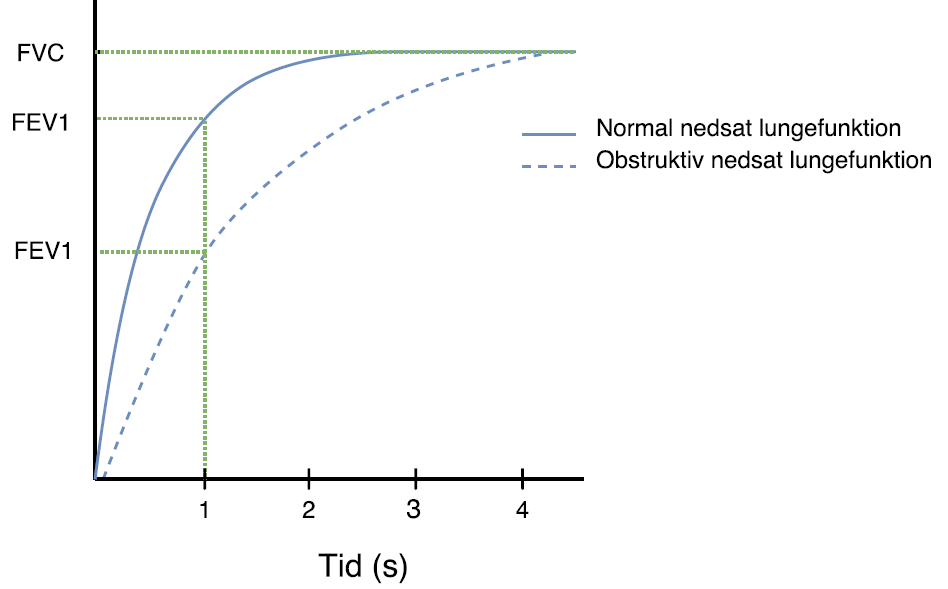
\includegraphics[width=0.5\textwidth]{figures/FEV}
\caption{Spirometrimåling ** MANGLER TEKST** MIDLERTIDIGT BILLEDE **}
\label{fig:FEV}
\end{figure} 

\noindent
Foruden lungefunktionsundersøgelser måles BMI, og der tages røntgen af thorax, EKG-målinger og blodprøver \cite{Sundhed2013}.
Med tiden kan symptomerne på KOL forværres, og der skal mindre fysisk aktivitet til for at udløse åndenød. \cite{Basisbogen2016}

\subsubsection{Klassifikation af KOLs sværhedsgrad}
Til vurdering af patientens symptomer anvendes blandt andet patienten egne erfaringer og vurderinger i forhold til livskvalitet med hensyn til sygdommens påvirkning i dagligdagen. Hertil anvendes Medical Research Council åndenødsskala (MRC) og COPD assessment test (CAT).
 
MRC-skalaen er en skala fra 1-5, hvor patienten vurderer mængden af aktivitet, der kan udføres i forhold til åndenød, der opleves. Skalaen kan ses på \ref{fig:MRC}, hvor 1 svarer til, at patienten først oplever åndenød under meget anstrengelse, og 5 svarer til, at patienten oplever åndenød ved meget lav aktivitet.

\begin{figure} [H]
\centering
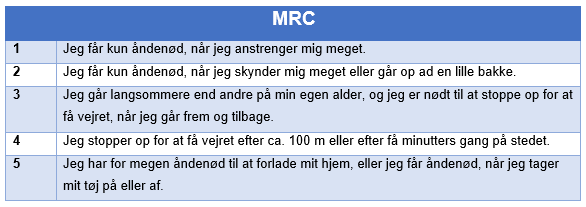
\includegraphics[width=0.9\textwidth]{figures/MRC}
\caption{MRC-skala ** MANGLER TEKST** MIDLERTIDIGT BILLEDE ** \cite{Basisbogen2016}}
\label{fig:MRC}
\end{figure} 

\noindent
CAT-scoren opnås ud fra patientens egne vurderinger af symptomer, såsom slim i lunger, hoste og åndenød. Patienten vurderer symptomerne fra 0 til 5. Jo højere den samlede score er, des værre vurderes symptomerne af patienten. \cite{Basisbogen2016}
 
Sværhedsgraden af KOL klassificeres af Dansk Selskab for Almen Medicin (DSAM) ud fra retningslinjer opstillet af the Global Initiative for Chronic Obstructive Lung Disease (GOLD). Hertil kan patienterne inddeles i fire forskellige kategorier; A, B, C og D, afhængig af antal eksacerbationer det seneste år, MRC, CAT-score samt lungefunktionstest.\cite{dsam2016} En inddeling af kategorierne kan ses på \ref{fig:CAT} .

\begin{figure} [H]
\centering
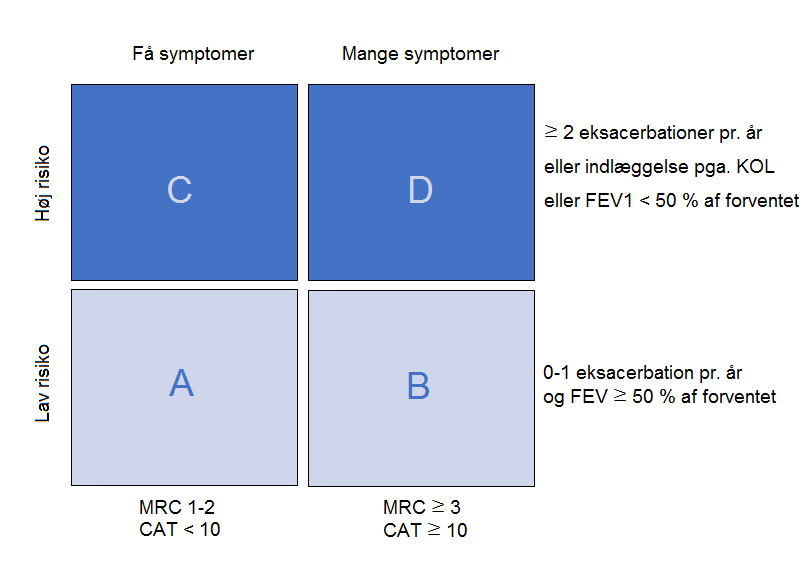
\includegraphics[width=0.5\textwidth]{figures/CAT}
\caption{CAT ** MANGLER TEKST** MIDLERTIDIGT BILLEDE ** \cite{Basisbogen2016, Sundhed2013}
\label{fig:CAT}
\end{figure} 

Sværhedsgraden af KOL kan også klassificeres udelukkende ud fra spirometrimålinger. Sværhedsgraderne inddeles i fire GOLD-stadier, som kan ses af \ref{fig:GOLD}.

\begin{figure} [H]
\centering
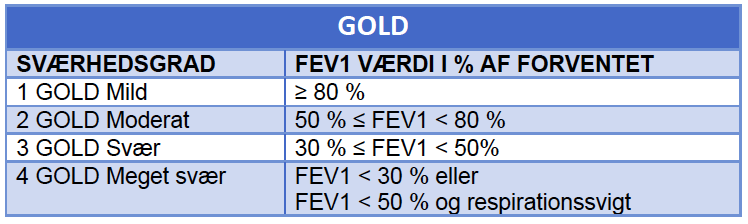
\includegraphics[width=0.5\textwidth]{figures/GOLD}
\caption{GOLD-stadier ** MANGLER TEKST** MIDLERTIDIGT BILLEDE ** \cite{Basisbogen2016, Sundhed2013}}
\label{fig:GOLD}
\end{figure} 

\subsection{Behandling}
Den eneste mulighed for at forhindre, at lungefunktionstabet accelererer yderligere, er ved rygestop eller ved ophør af eksponering af/til (?) den faktor, der er årsag til sygdommen.
Behandlingen af KOL kan inddeles i non-farmakologisk og farmakologisk. Non-farmakologisk behandling kan indebære hjælp til rygestop, eksempelvis ved brug af nikotinpræperater og gratis kommunale rygestopvejledninger. Det anbefales, at patienter med en MRC på 3 eller over udfører fysisk aktivitet som rehabilitering, og patienter med en BMI under 20 bør desuden deltage i ernæringsrådgivning. Patienter med sekretproblemer kan efter behov anvende CPAP (continous positive airway pressure) eller PEP-fløjte (positive expiratory pressure), enten i hjemmet eller på sygehus.
Den farmakologiske behandling består af bronkodilaterende inhalationsbehandling, som afhænger af graden af KOL. Yderligere kan antiinflammatorisk behandling gives til patienter med hyppige eksacerbationer. \cite{Basisbogen2016}
 
\subsection{Livskvalitet}
Prognosen for KOL-eksacerbation efter indlæggelse er der en dødelighed på næsten 10 \% i løbet af den første måned. Dødstallet ligger på omkring 64 per 100.000 per år for mænd og 54 per 100.000 per år for kvinder.
Hastigheden hvormed sygdommen progredierer for KOL patienter er specielt afhængig af, om patienten ophører med rygning og/eller eksponering til den udløsende faktor, og det er derfor vigtigt at få en tidlig diagnosticering, således at patienten hurtigt kan få hjælp og dermed få så god en prognose som muligt. \cite{dsam2016}
Et studie af har vist, at KOL patienter, der er i stadie 4 i GOLD-klassificeringen, har lav funktionalitet og livskvalitet, som bliver værre med tiden og ved fremkomst af flere symptomer til sygdommen. \cite{Habraken2011}

Der er en række komorbiditeter, som hyppigt ses hos KOL patienter, som desuden kan have en negativ påvirkning på patienternes livskvalitet og prognose. Ved årskontroller bør patienten tjekkes for de hyppigste komormiditeter; hjerte-kar-sygdomme, type-2 diabetes, osteoporose, lungecancer, muskelsvækkelse samt angst og depression.
Nogle af komorbiditeterne kan skyldes, at åndenød har medført et nedsat fysisk aktivitetsniveau og dermed svage perifere muskler. Desuden har rygning og generelt dårlig livsstil også betydning for udviklingen af disse komorbiditeter. \cite{dsam2016}
Psykiske komorbiditeter, ofte i form af depression og angst, har en øget forekomst hos patienter med en FEV1 værdi på under 50 \% af den forventede værdi, svarende til en GOLD-klasssificering på 3-4. Desuden kan angst og depression udløses ved diagnosen af KOL. Den øgede risiko for psykiske lidelser skyldes, at KOL kan medføre social isolation og tab af sociale relationer, skyldfølelse, usikkerhed med hensyn til fremtiden mm. \cite{dsam2016}
Fysisk aktivitet, rehabilitering samt non-farmakologisk og farmakologisk behandling har positiv effekt på nogle har disse komorbiditeter. \cite{dsam2016}
